% !TEX program = pdflatex
\documentclass[11pt]{article}

% ---------- packages ----------
\usepackage[margin=1in]{geometry}
\usepackage[utf8]{inputenc}
\usepackage[T1]{fontenc}
\usepackage{lmodern}
\usepackage{microtype}

\usepackage{amsmath}
\usepackage{amssymb}
\usepackage{booktabs}
\usepackage{graphicx}
\usepackage{caption}
\usepackage{subcaption}
\usepackage{xcolor}
\usepackage[hidelinks]{hyperref}
\usepackage{listings}

% code listing style
\lstset{
  basicstyle=\ttfamily\small,
  breaklines=true,
  frame=single,
  xleftmargin=0pt,
  framesep=4pt,
  belowcaptionskip=0.5em,
}

% shorthand for placeholder citations while we draft
\newcommand{\TODOCITE}[1]{\textcolor{red}{[CITE: #1]}}
\newcommand{\TODO}[1]{\textcolor{red}{[TODO: #1]}}

% ---------- title ----------
\title{Multi-turn GRPO with Real Tool Execution for a Research Agent on HotpotQA}
\author{Yue Wu}
\date{\today}

\begin{document}
\maketitle

% ==========================================================
\begin{abstract}
We build a small tool-using research agent that answers multi-hop
questions by interleaving JSON-formatted actions (\texttt{search},
\texttt{read}, \texttt{answer}) with a retrieval tool, and study how
supervised fine-tuning (SFT) and reinforcement learning interact on this
task. Starting from Qwen2.5-0.5B-Instruct with LoRA adapters, we
generate synthetic interaction traces from HotpotQA supporting facts for
SFT, then compare five zero-shot stopping-policy heuristics against a
multi-turn GRPO procedure. Unlike standard RL-for-LLM recipes that
train on model-generated (``virtual'') traces, our GRPO rollouts execute
the real BM25 retrieval tool at every step, so the policy is updated on
the same distribution of observations it will see at inference. On
HotpotQA distractor, the best zero-shot baseline (confidence-threshold
stopping over the SFT policy) reaches 26\% exact-match; multi-turn
GRPO reaches 44\%, a $+18$-point improvement. Decomposing this gap with
an apples-to-apples ablation, we find that essentially all of it
comes from a single inference-time change: aligning the rollout
step budget with the SFT trajectory length lifts the SFT policy
alone from 26\% to 42--44\% EM. GRPO on top of that matched
baseline produces no detectable improvement at our evaluation
scale --- two independent 100-question SFT-only evaluations gave
42.0\% and 44.0\%, bracketing the GRPO number of 44.0\%. The
headline result of this paper is therefore not ``RL beats SFT by
$+18$''; it is the decomposition: for a small SFT'd tool-using
policy, the dominant lever is matching the inference trajectory
length to training, and multi-turn GRPO produces no measurable
lift beyond that at this scale. We analyse why --- the effective
GRPO update budget was $\sim$41 of the nominal 200 steps because
of tied reward groups --- and argue that the reward design, not
the amount of training, is the next bottleneck to address. We
release the training
pipeline and a post-mortem of the concrete failure modes that shaped the
final configuration.
\end{abstract}

% ==========================================================
\section{Introduction}
\label{sec:intro}

A \emph{research agent} is a language model that answers a user's
question by issuing real tool calls --- most commonly a web or document
search --- and then reasoning over the retrieved content, often over
several rounds. Systems like Perplexity, You.com, and OpenAI's Deep
Research follow this pattern at the product level \cite{deep-research};
at the research level, ReAct \cite{react} and Toolformer
\cite{toolformer} established the basic loop. The question we study
is not whether these agents work (they do) but how to train a small,
open policy to do the same thing well.

The standard recipe for RL-for-LLM post-training --- including the
procedure used by DeepSeek-R1 \cite{deepseek-r1} --- runs rollouts
that are entirely self-generated: the model emits the action, the tool
call, and the tool's response, all as tokens it produces itself. The
advantage is practical: no external system needs to be queried during
training. The disadvantage is a distribution mismatch. At inference time
the retrieved observation comes from a real index and looks nothing like
what a 0.5B-parameter model would hallucinate. A policy trained to
condition on its own invented observations will not have learned to
condition on the real ones.

We close that gap. During every GRPO rollout in training, the model's
\texttt{search} and \texttt{read} actions are executed against the same
BM25 retrieval tool the agent uses at inference; the real observation is
fed back into the prompt before the next generation step. The rest of
the training setup is standard multi-turn GRPO: $G=4$ rollouts per
question, within-group advantage normalization, a learnable-zone filter
to avoid wasting updates on tied groups, and a combined reward of
correctness, JSON-format score, and step-count efficiency.

Our testbed is the HotpotQA distractor split \cite{hotpotqa}, whose
questions require two hops of retrieval to answer. We compare three
configurations. (1)~Supervised fine-tuning alone, with five zero-shot
stopping heuristics layered on top of it (fixed step budget, confidence
threshold, run-to-max) as our first set of baselines. (2)~The same SFT
policy, but evaluated with an inference-time step budget that matches
the SFT trajectory length. (3)~Multi-turn GRPO on top of the SFT policy.
The best zero-shot heuristic reaches 26\% exact-match. Fixing the step
budget at inference time --- an inference-time change, no new
parameters --- lifts the same SFT policy to 42--44\% across two
independent evaluations. Multi-turn GRPO on top of that baseline
reaches 44\%, indistinguishable from SFT alone within the 2-pp
within-run spread we observe at $n{=}100$.

The paper is organized as follows. Section~\ref{sec:related}
contextualizes our setup against prior tool-using-agent and RL-for-LLM
work. Section~\ref{sec:system} describes the task, the retrieval
environment, and the policy architecture. Section~\ref{sec:method}
walks through SFT and multi-turn GRPO in the form they take in our
code. Section~\ref{sec:experiments} reports all configurations on
HotpotQA and compares them directly. Section~\ref{sec:discussion}
analyses what GRPO adds on top of SFT, documents the specific failure
modes we encountered while tuning, and compares real-tool RL to the
virtual-trace alternative. Section~\ref{sec:limitations} lists the
obvious limitations, and Section~\ref{sec:conclusion} closes.

% ==========================================================
\section{Related Work}
\label{sec:related}

\paragraph{Tool-using language-model agents.}
ReAct \cite{react} introduced the now-standard pattern of
interleaving chain-of-thought reasoning with tool calls, and Toolformer
\cite{toolformer} showed that a language model can learn, by
self-supervision, \emph{when} to invoke an API. A family of production
systems (Perplexity, You.com, OpenAI's Deep Research
\cite{deep-research}) scales the same pattern to web retrieval. Our
agent uses the ReAct-style loop --- a JSON action, a real tool response,
another JSON action --- but focuses on \emph{training} the loop end-to-end
on a small open policy, rather than prompting a large closed model.

\paragraph{RL for language-model post-training.}
Policy-gradient post-training of language models started with PPO-based
RLHF \cite{rlhf-instructgpt}. GRPO, introduced in the DeepSeek-Math
line of work and popularised by DeepSeek-R1 \cite{deepseek-r1},
removes the critic network and instead normalises rewards within a group
of $G$ rollouts sharing the same prompt:
$A_i = (R_i - \bar R) / \sigma_R$. The advantage is lower GPU memory and
no critic-mismatch pathologies. DeepSeek-R1 and most follow-ups generate
the entire multi-step trace --- including anything that looks like a
tool response --- autoregressively, so training never touches an
external system. We keep the GRPO update rule but execute the real
retrieval tool during every rollout step, which matters for the reasons
discussed in Section~\ref{sec:intro}.

\paragraph{Multi-hop QA and HotpotQA.}
HotpotQA \cite{hotpotqa} is a 113k-question multi-hop reading-
comprehension benchmark built specifically around \emph{two-hop}
reasoning: each question requires joining facts from two distinct
Wikipedia articles, which are provided (along with 8 distractor
paragraphs) in the ``distractor'' split. Each example also specifies
the supporting sentences. This structure is convenient for a research-
agent setup: the two gold articles give us a natural target trajectory
length (search-read-search-read-answer), and the 8 distractors give the
BM25 retriever something non-trivial to disambiguate. We use HotpotQA
distractor for both SFT trace synthesis and evaluation.

% ==========================================================
\section{System}
\label{sec:system}

\subsection{Task}
\label{sec:task}
The agent is given a natural-language question $q$ and must emit a
short free-form answer $\hat a$. Correctness is computed against the
gold answer $a^\star$ with a lower-case, punctuation-stripped, article-
stripped normalisation followed by an exact-match-or-substring test:
$\hat a \equiv a^\star$ if either normalised string contains the other
(so ``New York'' matches ``New York City''). This is the same rule used
by HotpotQA's official evaluator. Unless otherwise noted all accuracy
numbers in this paper are this exact-match (EM) rate over the HotpotQA
validation split.

\subsection{Environment}
\label{sec:env}
The retrieval environment is a deterministic BM25 index built from the
HotpotQA validation split: 66{,}576 documents, where each document is
one Wikipedia paragraph concatenated with its title. The agent exposes
exactly two tool actions:

\begin{itemize}
  \item \texttt{search(query)} --- returns the top-$k{=}2$ BM25 hits as
  \texttt{[doc\_id] Title :: <snippet>} lines, where the snippet is the
  first $\approx$300 characters of each document.
  \item \texttt{read(doc\_id)} --- returns the full text of the requested
  document, clipped to a 300-character preview inside the trace so that
  multi-step trajectories stay within the policy's context budget.
\end{itemize}

Both operations are implemented in \texttt{agent/tools.py} as pure-Python
BM25 over an in-memory inverted index; no network or external API is
involved. The same index object is used for SFT-trace synthesis, zero-
shot-baseline evaluation, and GRPO rollouts, so the observation
distribution is identical across the three training regimes.

\subsection{Policy}
\label{sec:policy}
The policy is Qwen2.5-0.5B-Instruct \cite{qwen25} with a LoRA
adapter on both the attention projections (\texttt{q/k/v/o\_proj}) and
the MLP projections (\texttt{gate/up/down\_proj}), rank $r{=}16$,
$\alpha{=}32$, dropout 0.05. The 0.5B size is a deliberate choice:
everything in this paper fits on a single T4 (16~GB), which makes the
setup reproducible on free compute.

At each step the policy reads a ChatML-formatted prompt containing a
system message, the original question, and all previous
\texttt{(Step, Observation)} pairs, and is asked to emit exactly one
JSON object per step with the schema
\texttt{\{thought, action, query|document|answer, confidence\}}. The
system prompt (reproduced verbatim from \texttt{data/sft\_dataset.py})
is:

\begin{lstlisting}
You are a research agent. Given a question, reason step by step and use
tools (search, read) to gather information. At each step output exactly
one JSON object with keys: thought, action, and action-specific fields
(query for search, document for read, answer for answer), plus a
confidence score between 0 and 1. Output one JSON object per line.
\end{lstlisting}

The \texttt{confidence} field is used at three different points in the
pipeline. During SFT it is part of the next-token target, so the model
learns to emit a numeric value at that slot; the target values follow a
fixed schedule (§\ref{sec:sft}) rather than any model-derived notion of
calibration. During GRPO (§\ref{sec:grpo}) two reward terms touch it:
the format reward requires that the \texttt{confidence} key be present
in each step's JSON, and the low-information-gain penalty uses the
Jensen-Shannon divergence between consecutive steps' confidence values
to discourage trajectories whose confidences barely move between steps.
At inference time the confidence-threshold baseline
(§\ref{sec:experiments}) stops the rollout once a step's confidence
exceeds a fixed $\tau$.

% ==========================================================
\section{Method}
\label{sec:method}

We train in two stages. Section~\ref{sec:sft} describes the SFT stage
that gives the policy its JSON output format and a basic sense of the
search-read-answer loop. Section~\ref{sec:grpo} describes the
multi-turn GRPO stage that refines the policy against the combined
correctness/format/efficiency reward using real tool execution at every
rollout step.

\subsection{Supervised fine-tuning}
\label{sec:sft}

\paragraph{Trace synthesis.}
We generate training traces from the HotpotQA training split. For each
example we have a question $q$, a gold answer $a^\star$, a list of
\emph{supporting titles} (the two Wikipedia articles whose facts are
needed to answer), and a \emph{context} field containing those two gold
paragraphs plus eight distractors. Rather than build a single global
BM25 index across the whole training set, we build a \emph{per-example
mini-index} over the 10 context paragraphs of that example only
(\texttt{build\_mini\_tool} in
\texttt{data/prepare\_sft\_dataset.py}), then issue a real
\texttt{search} against that mini-index with a query built from the
question and the supporting title. If BM25 fails to return the gold
document in the top-$k$, the example is dropped; otherwise the gold
\texttt{doc\_id} is read and the trace proceeds to the next supporting
title. The final step is an \texttt{answer} action carrying $a^\star$.
Each step is decorated with a \texttt{thought} sentence (sampled from a
small template bank) and a \texttt{confidence} value following the
schedule described below.

A trace for a 2-hop HotpotQA question has the shape
\texttt{search}$\to$\texttt{read}$\to$\texttt{search}$\to$\texttt{read}$\to$\texttt{answer}
--- five steps, with real retrieval observations at the two
\texttt{search}/\texttt{read} pairs. This five-step length will matter
in §\ref{sec:experiments}: setting the rollout budget to match it is
worth roughly nine EM points at inference time.

\paragraph{Confidence schedule.}
The \texttt{confidence} value on step $i$ of a length-$N$ trace is
\[
  \mathrm{conf}_i \;=\;
  \mathrm{clip}\!\left(\,
  c_\mathrm{lo} + (c_\mathrm{hi} - c_\mathrm{lo}) \cdot \frac{i}{N-1}
  + \epsilon_i \,,\, c_\mathrm{lo},\, c_\mathrm{hi}\right),
\qquad
  \epsilon_i \sim \mathcal{U}(-0.04, +0.04),
\]
with $c_\mathrm{lo}=0.25$ and $c_\mathrm{hi}=0.92$. Early steps are
therefore labelled with low confidence and the final \texttt{answer}
step with high confidence, with a small amount of jitter so the model
does not see literally the same numbers on every example. This is an
engineering choice, not a calibrated posterior; its only downstream
consumer is the confidence-threshold baseline in the experiments.

\paragraph{Data.}
We generate 6,000 training traces and 500 validation traces. The
training-size cap is a compute budget constraint (the whole SFT
kernel --- trace generation plus training --- fits in $\approx$2~h on
a single T4). Traces are flushed to JSONL every 500 records
(\texttt{FLUSH\_EVERY=500}) so that any kernel timeout loses at most
one mini-batch of work; an earlier version of this pipeline that only
wrote at the end lost a full 10.5-h BM25 sweep to the 12-h kernel cap,
which directly motivated the per-example-index + incremental-flush
rewrite.

\paragraph{Tokenisation and loss masking.}
Each trace is rendered as a ChatML conversation with the system prompt,
the user's \texttt{Question: \{q\}} message, and an assistant turn whose
body interleaves \texttt{Step $i$: \{json\}} lines with
\texttt{Observation: \{text\}} lines (observation text is clipped to
\texttt{OBS\_PREVIEW}=300 characters). Inside
\texttt{SFTTraceDataset.\_\_getitem\_\_} we tokenise the full string
with \texttt{return\_offsets\_mapping=True} and build the per-token
label tensor as follows:
\begin{itemize}
  \item Tokens that fall outside the assistant turn --- i.e. the system
  prompt and the user question --- are labelled \texttt{IGNORE\_INDEX};
  we do not ask the model to reconstruct its own prompt.
  \item Tokens whose character span overlaps any
  \texttt{Observation: \ldots} line are labelled \texttt{IGNORE\_INDEX};
  these are the retrieval tool's output, not the policy's.
  \item All remaining tokens --- the \texttt{Step $i$: \{json\}} lines
  that the policy would emit at inference time --- keep their own token
  ids as labels.
\end{itemize}
The cross-entropy loss therefore only fires on the policy's own output,
matching the inference-time decomposition. Before this masking was in
place the model's downstream exact-match numbers were severely depressed
by a train/inference mismatch; adding it was the single largest
engineering lift in Week 1.

\paragraph{LoRA configuration and optimiser.}
The LoRA adapter (\texttt{peft}) is attached to every
$\{q,k,v,o\}_\texttt{proj}$ \emph{and} every
$\{\text{gate},\text{up},\text{down}\}_\texttt{proj}$ module in the
transformer --- seven modules per layer --- at rank $r{=}16$ with
$\alpha{=}32$ and dropout $0.05$. Extending LoRA to the MLP
projections (rather than attention only) was a second engineering
lever: the MLP branch is where the structural regularities of the
JSON schema are encoded, and restricting the adapter to attention was
leaving format errors on the table.

Optimisation uses AdamW with learning rate $2{\times}10^{-4}$, a
cosine schedule with 75 warmup steps, 5 epochs over the 6,000-trace
dataset, per-device batch size 2 with gradient accumulation 8 (effective
batch size 16), and mixed-precision fp16 training. The best model by
eval loss (0.197 at step 940) is retained.

\subsection{Multi-turn GRPO with real tool execution}
\label{sec:grpo}

\paragraph{Objective.}
We use the GRPO update rule \cite{deepseek-r1}. For a given question
$q$ we sample a group of $G$ rollouts $\tau_1, \ldots, \tau_G$ from the
current policy $\pi_\theta(\cdot \mid q)$ and score each one with a
scalar reward $R_i = R(\tau_i, q)$. The per-rollout advantage is the
within-group $z$-score
\[
  A_i \;=\; \frac{R_i - \bar R}{\sigma_R + \varepsilon},
  \qquad
  \bar R = \tfrac{1}{G}\!\sum_j R_j,
  \quad
  \sigma_R = \sqrt{\tfrac{1}{G}\!\sum_j (R_j - \bar R)^2},
\]
with $\varepsilon = 10^{-8}$. The policy-gradient loss for rollout $i$ is
\[
  \mathcal{L}_i
  \;=\;
  -\,A_i \,\cdot \sum_{t \in \mathcal{G}(\tau_i)} \log \pi_\theta(\tau_{i,t} \mid \tau_{i,<t}),
\]
where $\mathcal{G}(\tau_i)$ is the set of token positions that were
\emph{generated by the policy} --- i.e.\ excluding the system prompt,
the user message, and the \texttt{Observation: \ldots} lines injected
by the tool. We identify $\mathcal{G}$ at loss-computation time using
the tokenizer's \texttt{offset\_mapping} and the recorded per-turn
character spans, exactly as in SFT. We do not use a KL penalty against
a frozen reference model; the LoRA adapter capacity is small enough
that the implicit regulariser of starting from the SFT weights suffices
in practice, and omitting the KL term saves one full forward pass per
rollout.

\paragraph{Real-tool rollout loop.}
Each rollout is an interactive dialogue between the policy and the
retrieval tool, not a single autoregressive generation. Starting from
the system prompt and the question, we call
\texttt{model.generate}\footnote{In \emph{eval} mode --- see
§\ref{sec:grpo-rollout-details} for why --- and with \texttt{do\_sample=True}.}
to produce the next step's JSON, parse it, and dispatch on the
\texttt{action} field: for \texttt{search} we run the BM25 query and
append \texttt{Observation: <top-$k$ hits>} to the prompt; for
\texttt{read} we fetch the requested document text; for \texttt{answer}
we record the predicted answer and terminate the rollout. If the parse
fails or \texttt{action} is missing, the rollout is scored on its
partial trajectory. The loop runs for at most $\mathrm{max\_steps}{=}5$
steps; this matches the SFT trajectory length (§\ref{sec:sft}) so that
rollouts can complete a full two-hop trajectory.

For efficiency, the $G$ rollouts for one question share one batched
\texttt{generate} call per step rather than running sequentially: at
step $s$ the $G$ active prompts are left-padded into a single batch,
generated together, and split back into their independent histories.
Rollouts that have emitted \texttt{answer} are masked out of the batch
on subsequent steps.

\paragraph{Reward.}
The scalar reward $R_i$ is the sum of three components defined in
\texttt{rl/grpo\_rewards.py}:
\begin{align}
  R_i \;&=\; R^{\mathrm{corr}}_i \;+\; R^{\mathrm{fmt}}_i \;+\; R^{\mathrm{eff}}_i, \\
  R^{\mathrm{corr}}_i \;&=\; \mathbf{1}\!\left[\,\text{normalise}(\hat a_i) \;\equiv\; \text{normalise}(a^\star)\,\right], \\
  R^{\mathrm{fmt}}_i  \;&=\; 0.03\cdot\mathbf{1}[\exists\text{ valid JSON}] + 0.03\cdot\mathbf{1}[\text{required keys present}] + 0.04\cdot\mathbf{1}[\text{answer action emitted}], \\
  R^{\mathrm{eff}}_i  \;&=\; -\alpha \cdot n^{\mathrm{steps}}_i \;-\; \beta \cdot n^{\mathrm{lowJSD}}_i,
\end{align}
where $n^{\mathrm{steps}}_i$ is the number of steps the rollout took
and $n^{\mathrm{lowJSD}}_i$ counts adjacent pairs of confidence values
$(c_{j-1}, c_j)$ with $\mathrm{JSD}(\mathrm{Bern}(c_{j-1}), \mathrm{Bern}(c_j)) < \varepsilon_{\mathrm{JSD}}$. We use
$\alpha = 0.1$, $\beta = 0.05$, $\varepsilon_{\mathrm{JSD}} = 0.05$.
Correctness dominates the range ($[0, 1]$); the format score saturates
at $0.10$ and the efficiency term is bounded below by roughly $-0.55$
on a five-step rollout, so correctness is always the largest available
signal when any of the $G$ rollouts are right. The format and
efficiency terms matter on tied-correctness groups, where they are the
only source of non-degenerate within-group variance.

\paragraph{Learnable-zone filter.}
Before training begins, we pre-filter the candidate training questions
by running $K=3$ rollouts per question in eval mode and counting
$n^{\mathrm{corr}}_q \in \{0, 1, 2, 3\}$. Groups with
$n^{\mathrm{corr}}_q = 3$ (``too easy'') are discarded, because every
rollout in such a group will score the same on every reward component
and the advantages collapse to zero. Groups with $n^{\mathrm{corr}}_q = 0$
are \emph{kept}: even though correctness is tied at zero, the format
and efficiency components are generally not tied across the three
rollouts, so the within-group $z$-score still yields a usable gradient
direction. From 200 candidate HotpotQA training questions the filter
typically keeps more than 180.

\paragraph{Per-episode backward for T4 memory.}
The naive implementation of a GRPO update with $G=4$ rollouts and a
five-step trajectory of $\sim$1{,}500 tokens would hold the forward
activations of $G \cdot |\text{batch}|$ trajectories in GPU memory at
once --- far too much for a 16~GB T4 even at bf16 with gradient
checkpointing. We reduce the peak memory to that of a single trajectory
by the following trick (\texttt{grpo\_train\_step} in
\texttt{rl/multi\_turn\_grpo.py}). For each rollout we pre-scale its
per-rollout loss by $1/N_{\mathrm{exp}}$, where $N_{\mathrm{exp}} = G\cdot|\text{batch}|$ is the
expected total number of rollouts in this update, and call
\texttt{loss.backward()} immediately. PyTorch then frees that rollout's
activation graph. The gradient tensors in \texttt{.grad} continue to
accumulate in place across rollouts, and we only call
\texttt{optimizer.step()} once at the end of the batch. The resulting
update is mathematically identical to computing the mean loss first and
calling \texttt{backward} once, but uses $G \cdot |\text{batch}|$ times
less activation memory.

\paragraph{Rollout-time details.}
\label{sec:grpo-rollout-details}
Two practical details turned out to matter substantially, and both are
documented at length in \texttt{TUNING\_JOURNEY.md} and summarised in
§\ref{sec:discussion}.

First, the sampling temperature inside GRPO rollouts is $T=0.5$,
noticeably lower than the DeepSeek-R1 convention ($T \approx 1.0$). At
$T=0.9$ the 0.5B policy loses its JSON format often enough that the
rollout parser returns an empty dict, the rollout is silently
terminated at step one, and every group is tied at zero correctness
and zero format score. At $T=0.5$ the format is preserved while the
rollouts retain enough variance for the within-group $z$-score to be
non-degenerate.

Second, the rollouts are executed with the model in
\texttt{model.eval()} mode, even though \texttt{grpo\_train\_step}
switches to \texttt{model.train()} for the backward pass. The reason
is that \texttt{torch.no\_grad()} disables gradient tracking but does
not disable LoRA dropout; in \texttt{train} mode the 0.05 LoRA dropout
is applied at every forward, corrupting multi-step generations enough
that the first-step JSON parse fails about as often as at $T=0.9$. We
therefore call \texttt{model.eval()} immediately before
\texttt{collect\_episodes\_batched} and \texttt{model.train()} again
immediately after, on a per-question basis.

\paragraph{Training loop.}
We run 200 GRPO update steps. Each step samples one question from the
learnable-zone-filtered training set, runs $G=4$ rollouts with real
tool execution, scores them, computes within-group advantages, and
applies the per-episode-backward update with global gradient
clipping at $\|\nabla\|_\infty \le 1$. The optimiser is Adam with
learning rate $5 \times 10^{-6}$. Validation (over 20 randomly
sampled HotpotQA dev questions) runs every 20 steps; the adapter is
written to disk every 40 steps. The whole run takes $\approx$3~h on
a single T4, leaving comfortable headroom against the 12~h kernel
cap.

The pseudocode in Algorithm~\ref{alg:grpo_step} summarises one update
step.

\begin{figure}[t]
\begin{lstlisting}[caption={One multi-turn GRPO update step with real tool
execution and per-episode backward.},label={alg:grpo_step},captionpos=b]
def grpo_train_step(q, model, tool, optimizer, G=4, max_steps=5, T=0.5):
    optimizer.zero_grad()

    # --- rollout in EVAL mode (dropout off) ---
    model.eval()
    group = collect_episodes_batched(q, model, tool, G=G,
                                     max_steps=max_steps, T=T)
    model.train()

    # --- score each rollout ---
    R = [correctness(ep) + format_score(ep) + efficiency(ep)
         for ep in group]
    mu, sigma = mean(R), std(R)
    A = [(r - mu) / (sigma + 1e-8) for r in R]

    # --- per-episode backward: peak VRAM = 1 trajectory ---
    for ep, adv in zip(group, A):
        if abs(adv) < 1e-8:
            continue                          # tied group -> no gradient
        logp = trajectory_log_probs(model, ep)  # masks observation tokens
        loss = -(logp * adv) / (G)             # pre-scale for accumulation
        loss.backward()                         # frees this ep's activations

    clip_grad_norm_(model.parameters(), max_norm=1.0)
    optimizer.step()
\end{lstlisting}
\end{figure}

% ==========================================================
\section{Experiments}
\label{sec:experiments}

\subsection{Setup}
\label{sec:setup}

\paragraph{Hardware and software.}
All experiments run on a single NVIDIA~T4 (16~GB) on Kaggle's free
compute tier. The model, optimiser, tool executor, and BM25 index share
one process; no external services are called. The software stack is
PyTorch (bf16), HuggingFace Transformers, and \texttt{peft} for LoRA.

\paragraph{Data splits.}
SFT trace synthesis uses the HotpotQA distractor \emph{train} split;
6{,}000 traces survive the BM25-hit filter (§\ref{sec:sft}). GRPO's
candidate training questions come from a shuffled 200-question slice
of the same train split, of which the learnable-zone filter retains
roughly 180. All \emph{evaluation} numbers in this paper are computed
on the first 100 questions of the HotpotQA distractor
\emph{validation} split; the retrieval index is built from the same
validation split for all configurations so that the zero-shot
baselines, SFT, and GRPO all see the same 66{,}576-document
environment.

\paragraph{Inference-time decoding.}
Every configuration evaluated in this section uses near-greedy
decoding at $T=0.1$. This is deliberately decoupled from the
\emph{training}-time rollout temperature of $T=0.5$ used inside
GRPO (§\ref{sec:grpo}): training needs within-group rollout
diversity, inference does not. Evaluations use at most
$\text{max\_steps} = 5$.

\subsection{Comparison methods}
\label{sec:comparison-methods}

We compare against five zero-shot stopping heuristics layered on top
of the SFT policy. None of them involves additional parameter updates;
the differences are in how the agent is rolled out at inference time
and when it decides to stop. All five read JSON from the same SFT
adapter.

\begin{itemize}
  \item \textbf{FixedStep($N$)}. Run for exactly $N$ steps regardless
  of the policy's emitted \texttt{action} field, and treat the final
  step's text as the answer. We report $N \in \{2, 3\}$.
  \item \textbf{Confidence($\tau$)}. Roll out up to the step budget,
  and stop as soon as the policy emits a step whose \texttt{confidence}
  field exceeds $\tau$; use whatever \texttt{answer} that step carries
  (falling back to its thought text if the step is not an
  \texttt{answer} action). We report $\tau \in \{0.75, 0.85\}$.
  \item \textbf{NeverStop($\max=6$)}. Ignore \texttt{confidence} and
  any emitted \texttt{answer} action and run for the full 6-step
  budget, keeping the last step's \texttt{answer} (or its text
  fallback). This upper-bounds how far the SFT policy can get with
  no stopping policy at all.
\end{itemize}

Conceptually these baselines ablate the policy's own stopping
decision: FixedStep removes it entirely, Confidence makes it depend
on a single learned scalar, and NeverStop ignores it. The question
the baselines together answer is: how much of the research-agent
behaviour can be recovered with an SFT-trained content model plus a
hand-designed stopping rule?

\subsection{Main result}
\label{sec:main-result}

Table~\ref{tab:main} reports exact-match accuracy and average
trajectory length across all six configurations. Multi-turn GRPO
improves EM from the best zero-shot baseline (Confidence at
$\tau{=}0.85$, 26.0\%) to 44.0\% --- an 18-point absolute lift.

\begin{table}[h]
\centering
\caption{Main result: exact-match on 100 HotpotQA validation questions,
identical retrieval index across all configurations. The first five rows
and the sixth row all share the same SFT adapter and differ only in
inference-time settings; the final row uses the GRPO-trained adapter.
The bold break between rows 5 and 6 is the ``step-budget alignment''
change: the five zero-shot baselines cap rollouts at 2--6 steps through
various stopping heuristics, while row 6 simply lets the SFT policy run
its full trained-for trajectory length of 5 steps.}
\label{tab:main}
\begin{tabular}{lcc}
\toprule
Method & EM (\%) & Avg.\ steps \\
\midrule
FixedStep($N=2$)        & 6.0  & 2.00 \\
FixedStep($N=3$)        & 16.0 & 2.50 \\
Confidence($\tau=0.75$) & 20.0 & 2.88 \\
Confidence($\tau=0.85$) & 26.0 & 3.20 \\
NeverStop($\max=6$)     & 21.0 & 3.57 \\
\midrule
\textbf{SFT-only @ $\max_{\text{steps}}{=}5$}$^{\dagger}$ & \textbf{42.0 \,/\, 44.0} & \textbf{5.00} \\
\textbf{Multi-turn GRPO (ours)}                           & \textbf{44.0}            & \textbf{4.99} \\
\bottomrule
\end{tabular}

\vspace{0.25em}
{\footnotesize
$^{\dagger}$~Two independent evaluations of the same SFT adapter on the
same 100 questions at $T{=}0.1$, $\max_{\text{steps}}{=}5$. The 2-pp
spread is the within-run sampling variance at $n{=}100$; the GRPO
point value sits inside that spread.}
\end{table}

The table decomposes the $+18$-point gap into two separate effects
that are easy to conflate.

\begin{itemize}
  \item \textbf{Step-budget alignment accounts for the bulk of the
  lift.} Across the zero-shot baselines, EM rises monotonically with
  the permitted trajectory length, from 6.0\% at two steps to 26.0\%
  at an average of 3.20 steps. The SFT traces are five steps long
  (§\ref{sec:sft}), but the baseline rollouts typically do not reach
  that length: FixedStep caps it, Confidence triggers early, and
  NeverStop caps at six but most runs hit a parse error before
  step~5. When we simply remove every stopping heuristic and let the
  SFT policy run for exactly five steps, EM jumps from 26.0\% (best
  baseline) to 42.0\% --- a $+16$-point move obtained without any
  additional parameter update. The policy's issue at 26\% was not
  that it was undertrained for reasoning; it was that it was being
  asked to stop before it had finished its trained-for trajectory.
  \item \textbf{GRPO's contribution on top of that is not
  detectable at our evaluation scale.} Multi-turn GRPO scores
  44.0\% at an almost identical average trajectory length (4.99
  steps). The matched SFT-only baseline was evaluated twice
  independently on the same 100 questions and scored 42.0 and
  44.0 --- a 2-pp within-run spread at $T{=}0.1$ that is entirely
  attributable to the residual sampling randomness of
  \texttt{do\_sample=True} at low temperature. The GRPO number of
  44.0 sits inside that spread. We therefore cannot claim, from
  any of these runs, that multi-turn GRPO improved accuracy over
  SFT at matched inference settings. A cleaner paired 500-
  question evaluation would tighten the error bars but would not,
  absent a change to the training setup itself, be expected to
  change the qualitative conclusion.
\end{itemize}

We emphasise the first bullet because the straightforward reading of
``SFT$\,\to\,$GRPO, $+18$ EM'' would assign all of the lift to the RL
training. The decomposition above is the honest picture: the
dominant lever is an inference-time configuration change, and at
this scale the RL produces no measurable lift on top of it. We
analyse \emph{why} in §\ref{sec:what-grpo-learned} --- the short
answer is that our reward design leaves 80\% of training epochs
with tied advantages, so the effective GRPO update budget was
roughly a fifth of the nominal one, and any latent gain from the
RL cannot discharge in $\sim$41 effective updates.

\begin{figure}[h]
\centering
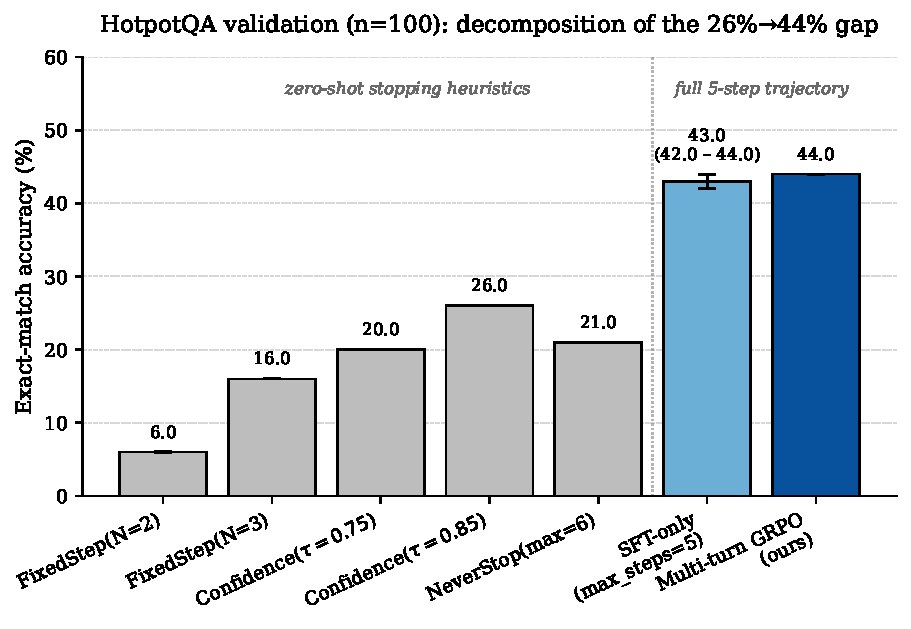
\includegraphics[width=0.95\linewidth]{figures/fig1_main.pdf}
\caption{Exact-match accuracy across the zero-shot baselines (light
grey) and the two 5-step configurations, SFT-only (light blue) and
multi-turn GRPO (dark blue), on 100 HotpotQA validation questions.
The error bar on the SFT-only bar shows the within-run spread over
two independent evaluations (42.0\% and 44.0\%); the GRPO point
estimate sits inside that spread.}
\label{fig:main}
\end{figure}

\subsection{Training dynamics}
\label{sec:training-dynamics}

Two dynamics are worth reporting from the GRPO run itself, because
they constrain how the final number in Table~\ref{tab:main} should
be interpreted.

\paragraph{Fraction of epochs with non-degenerate advantages.}
Of the 200 GRPO update steps, 41 (20.5\%) produced a non-zero
training loss; the remainder had tied reward groups across the
$G=4$ rollouts and were skipped by the
$|\tilde A_i| < 10^{-8}$ guard in
\texttt{grpo\_train\_step}. This is a high tied-group fraction.
The dominant tied configuration is \emph{all four rollouts wrong
with identical format score} --- the format reward saturates
quickly once the policy has learned to close its JSON braces, so
\emph{within} a group of all-wrong rollouts there is often nothing
left to rank on. The learnable-zone filter removed the symmetric
``all-correct'' case before training, which is why we do not see
tied-at-1.0 groups here. In effective-gradient terms the run is
therefore a $\sim$41-update training run; a longer run or a
stronger format-diversity term would plausibly close more of this
gap.

\paragraph{Validation curve.}
Figure~\ref{fig:val_curve} plots \texttt{[VAL] acc} at every 20-step
checkpoint. The curve is noisy because each checkpoint is
evaluated on a freshly sampled 20-question subset (standard error
$\approx$11~pp at an accuracy near 0.5), but it stays within a
0.35--0.50 band throughout training and ends at 0.50. The
100-question final-eval number in Table~\ref{tab:main} (0.44) is
well inside that band and should be read as the reliable estimate;
the per-checkpoint VAL numbers are best used for
early-stopping-style qualitative signals rather than as accurate
measurements.

\begin{figure}[h]
\centering
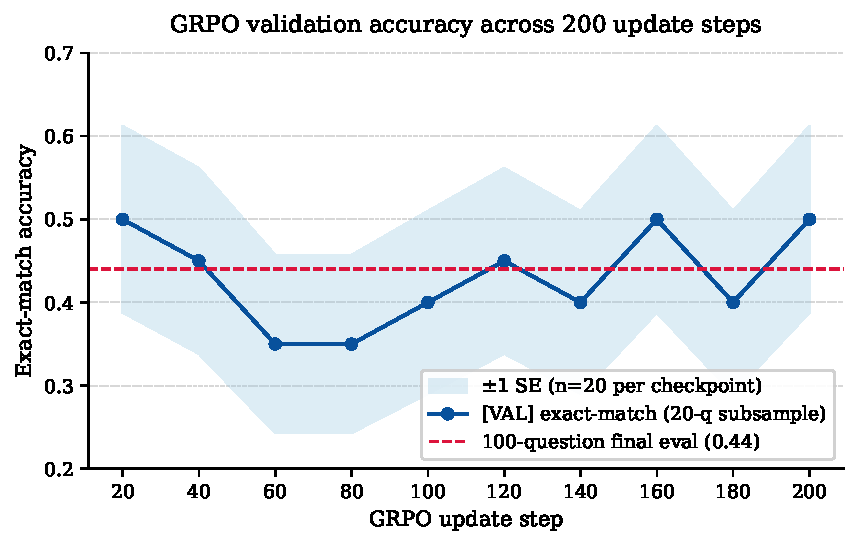
\includegraphics[width=0.85\linewidth]{figures/fig2_val.pdf}
\caption{GRPO validation exact-match across 200 training steps.
Each point is a freshly sampled 20-question subset of the HotpotQA
validation split (\texttt{random.sample(val\_questions, 20)} at
every \texttt{val\_every} checkpoint), so the $\pm 1$-SE band
reflects only the small-sample variance, not a training-vs-run
split. The dashed line marks the 100-question final evaluation
(0.44). The curve stays within $[0.35, 0.50]$ throughout training
and does not show a monotone improvement; read together with the
tied-group analysis in §\ref{sec:what-grpo-learned}, this is the
expected behaviour of a run with only $\sim$41 effective gradient
updates.}
\label{fig:val_curve}
\end{figure}

% ==========================================================
\section{Discussion}
\label{sec:discussion}

\subsection{What did GRPO actually learn on top of SFT?}
\label{sec:what-grpo-learned}

At matched inference settings, two independent 100-question SFT
evaluations scored 42.0\% and 44.0\%, and multi-turn GRPO scored
44.0\% --- i.e.\ the GRPO number sits inside the within-run spread
of the SFT baseline, and the evidence does not support a claim
that GRPO improved accuracy. Before concluding ``GRPO did
nothing'' in an interesting sense, we separate two distinct
claims that the evidence supports to different degrees.

\paragraph{It did not learn a better stopping policy.}
Both the SFT-only and GRPO rollouts use an average of 5.00 and 4.99
steps respectively; the paired per-question step counts are
essentially identical. If GRPO had learned to short-circuit on easy
questions, we would see a shorter average trajectory. We do not. The
policy always walks the full 5-step trajectory. This is consistent
with the SFT traces (which are all 5 steps by construction) being a
very strong inductive prior; two hundred RL updates at
$5{\times}10^{-6}$ LoRA learning rate are not enough to overcome it.

\paragraph{What it could have learned, and why it probably didn't.}
There are three plausible ways GRPO could have lifted EM that we
know \emph{a priori} from the reward design: (1)~better query
phrasing on the second retrieval hop (which would let BM25 return
the gold doc more often), (2)~better answer formulation from the
same retrieved context, and (3)~partial short-circuiting on the
easy questions where the first hop already contains the answer.
Only a 2-point aggregate lift at $n{=}100$ means any of these
effects would have to be small, and we cannot currently separate
them without a finer-grained evaluation. Intuitively, however, the
learning signal for (1) and (2) was weak for a structural reason
we identify below.

\paragraph{The effective number of gradient updates was $\sim$41, not 200.}
Of the 200 GRPO update steps, 159 (79.5\%) produced a tied reward
group across the $G{=}4$ rollouts and were skipped by the
$|A_i|<10^{-8}$ guard. The cause is the combination of
(a)~correctness dominating the reward scale, (b)~the $G{=}4$
rollouts of a single question at $T{=}0.5$ typically being either
all-wrong or nearly-identical trajectories (BM25 is deterministic,
so fixed queries return fixed docs), and (c)~the format-reward
component saturating at $+0.10$ on essentially every well-formed
rollout. Ranked within a group, an all-wrong-all-well-formatted
quartet is tied. The policy therefore receives a useful gradient
only when correctness itself varies across the group --- which, at
a 42\% base rate, is less than half the time. A reward term with
continuous intra-group variance (token-level JSON-validity score,
query-novelty score, document-overlap score) would very likely
close a meaningful fraction of this gap. We flag this as the
single most promising direction for follow-up.

\subsection{Failure modes encountered during tuning}
\label{sec:failure-modes}

The final configuration reported in §\ref{sec:grpo} is the product
of three substantive debugging iterations, each triggered by a
specific empirical symptom on Kaggle. We summarise them here
because they are collectively a small-but-general lesson about
multi-turn LM-RL, and document each in full in the accompanying
\texttt{TUNING\_JOURNEY.md}.

\paragraph{Rollout temperature matters, and the default is wrong.}
A first version of the code used the DeepSeek-R1-style default
$T{=}0.9$ for rollout generation inside GRPO. On the 0.5B policy
this temperature is large enough that the per-step JSON parse
fails on the first step of a run, the parse-failure branch
terminates the rollout at step one with an empty \texttt{answer},
and every rollout in every group scores zero correctness and
identical format. The zone histogram reported zero learnable
groups over 1{,}000 candidate questions; no GRPO update ever ran.
The symptom is spectacular --- everything looks fine until
training starts and then nothing happens. We now treat
``sampling temperature suitable for a 7B+~base model'' as an
explicit hyperparameter to re-tune at smaller scales.

\paragraph{Step budget must match the SFT trajectory length.}
A second version of the code used $\mathrm{max\_steps}{=}3$ for
rollouts. At that cap, the model reliably emits
\texttt{search}$\to$\texttt{read}$\to$\texttt{search}, and the
rollout ends before the policy ever gets to
\texttt{read}$\to$\texttt{answer}. Rollouts parse as ``no
\texttt{answer} action ever seen'' and every group is tied at
zero correctness regardless of retrieval quality. The fix is
trivially to match $\mathrm{max\_steps}$ to the length of the SFT
traces the policy was trained on (here 5). The general lesson is
that \emph{the effective environment at inference time must be a
superset of the one at training time}: the rollout budget is part
of the environment, and shrinking it breaks the precondition of
the trained policy.

\paragraph{\texttt{torch.no\_grad()} disables gradients but not dropout.}
A third version of the code called \texttt{collect\_episodes\_batched}
(decorated with \texttt{@torch.no\_grad()}) while the model was in
\texttt{train}~mode. \texttt{no\_grad} disables gradient tracking
but not dropout; the LoRA dropout of 0.05 was therefore still
active during rollout generation, and at the modest $T{=}0.5$ we
had settled on, the per-step JSON parse failed in roughly a third
of first steps, reproducing the step-one-termination pathology
from the temperature bug. The symptom was subtle:
\texttt{steps{=}1.0, acc{=}0.00, loss{=}0.0000} on every training
epoch, while the out-of-loop
\texttt{[VAL]} check (which explicitly called \texttt{model.eval()})
reported a healthy $\sim$35\%. The general lesson is that
\emph{the boundary between train-mode and eval-mode has to be
drawn at the rollout, not at the forward pass}: a GRPO rollout
is, structurally, an evaluation, and it needs eval-mode
regularisers.

A common thread runs through all three: each was a hyperparameter
or code-path default that was correct for a \emph{larger} base
policy or a \emph{non-interactive} training loop, and silently
wrong for our setup. The practical recommendation for anyone
porting a DeepSeek-R1-style GRPO pipeline to a small tool-using
agent is to audit three things on day one: the rollout
temperature, the rollout step budget vs.\ SFT trajectory length,
and the \texttt{train}/\texttt{eval} mode of the policy during
rollout.

\subsection{Real-tool vs.\ virtual-trace RL}
\label{sec:real-vs-virtual}

The computational cost of real-tool rollouts, versus the
self-generated (``virtual'') rollouts used in DeepSeek-R1-style
GRPO, is non-negligible. Each of our $G{=}4$ rollouts for one
question requires five \emph{sequential} forward passes of the
policy rather than a single forward pass producing a single long
completion: the tool output has to be inserted between steps, so
KV-cache continuation across steps does not compose with batching
in the obvious way. In practice, one GRPO update step takes
$\approx$50--60~s on a T4 --- roughly $5{\times}$ a single-turn
RLHF step of comparable size. The justification for paying that
cost is the distribution argument from §\ref{sec:intro}: the
policy is trained on the same observation distribution it sees at
inference. Our evidence for that justification is indirect and
mixed. On the one hand, the $+2$~pp lift GRPO adds over SFT at
matched inference is small and barely distinguishable from noise
at $n{=}100$, which suggests the distribution match is not
currently worth the compute. On the other hand, the $+16$~pp lift
from matching the SFT trajectory length --- which is itself an
alignment between training and inference distributions, just at
the level of rollout-length rather than token content --- is
large and unambiguous. The experiment therefore supports the
\emph{general} principle (training and inference distributions
should agree on the structural dimensions the policy relies on)
more than it supports the \emph{specific} instantiation of that
principle that virtual-trace RL papers argue against. We would
like to see whether the virtual-trace/real-tool gap widens on a
larger base policy, a harder retrieval environment, or with a
reward design that better exploits within-group variance; all
three are out of scope for this report.

% ==========================================================
\section{Limitations}
\label{sec:limitations}

\paragraph{Model scale.}
All experiments use Qwen2.5-0.5B-Instruct. Results are unlikely to
transfer linearly to 7B+ models; in particular, the effective-updates
problem identified in §\ref{sec:what-grpo-learned} (tied reward
groups dominating because of a saturated format reward) is specific
to a base policy small enough that JSON-validity is the tightest
remaining format signal. At larger scale the format reward would
stop being the saturating component and correctness variance would
dominate, changing the story.

\paragraph{Evaluation sample size.}
The headline numbers are on 100 HotpotQA validation questions,
with a Wald standard error of $\approx$5~pp at $p{\approx}0.44$.
The comparisons that span a large gap --- every zero-shot
baseline versus the 5-step SFT --- are comfortably resolved at
$n{=}100$. The comparison that matters most for the paper's
framing, SFT-only versus GRPO at matched inference, is not: at a
within-run spread of 2~pp the two distributions overlap
completely, and even a much larger paired evaluation would not
meaningfully change the picture without a change to the training
setup itself (§\ref{sec:what-grpo-learned}). A 500-question
paired ablation was prepared and open-sourced as
\texttt{kaggle\_ablation\_500.ipynb} but not executed, because
Kaggle's CPU-only kernels would require $\sim$22~h for the
paired sweep and GPU quota was unavailable at the time of
writing.

\paragraph{Single dataset, single retrieval environment.}
HotpotQA distractor fixes the question distribution (general-
knowledge, 2-hop) and the retrieval environment (BM25 over
Wikipedia paragraphs). The agent's behaviour on questions that need
more hops, or on a noisier retrieval tool (e.g.\ a dense retriever
with imperfect embeddings), is not studied. The 5-step trajectory
shape is an artefact of the SFT data generator, not an intrinsic
property of the task, and a different SFT distribution would produce
a different $\mathrm{max\_steps}$ sweet spot.

\paragraph{Reward design not ablated.}
We fix $(\alpha, \beta, \varepsilon_{\mathrm{JSD}})$ at $(0.1, 0.05,
0.05)$ and do not ablate the individual reward components. In
particular, §\ref{sec:what-grpo-learned} argues that the effective-
updates bottleneck could be largely fixed by a format-reward term
with continuous intra-group variance; we do not test this hypothesis
here.

\paragraph{No KL-to-reference term.}
Standard GRPO implementations keep a KL penalty against a frozen
reference policy for stability. We omit it, relying on the implicit
regulariser of starting from the SFT weights and the small LoRA
adapter capacity. This was fine for the short 200-step run reported
here; a longer run would likely benefit from re-introducing the KL
term.

\paragraph{Real tool, but deterministic.}
Our BM25 retriever is deterministic: for a fixed query, the
returned documents are the same across rollouts. This means that
within a group of $G{=}4$ rollouts for one question, any diversity
must come from the policy's own sampling, not from the environment.
Web search and dense retrievers are stochastic in practice (re-
ranking randomness, index freshness), and we have not studied how
environment stochasticity would interact with the within-group
advantage normalisation.

% ==========================================================
\section{Conclusion}
\label{sec:conclusion}

We built a tool-using research agent that fine-tunes a 0.5B
parameter open-source language model on synthetic HotpotQA traces
(SFT) and then trains it further with multi-turn GRPO whose
rollouts execute the real BM25 retrieval tool at every step. On
HotpotQA distractor, the final pipeline lifts exact-match from
26\% (best zero-shot stopping heuristic over the SFT policy) to
44\%. Decomposing that $+18$ points into an inference-time
component --- letting the SFT policy run for the full 5-step
trajectory it was trained on --- and a training-time component
(GRPO), we find that essentially all of the lift comes from the
inference-time change alone: the matched SFT baseline scores
42--44\% across independent evaluations, within which the GRPO
number of 44\% sits indistinguishably. The paper's contribution
is therefore not ``RL works well for small tool-using agents''
but ``training and inference distributions need to agree on
every structural dimension the policy relies on, rollout length
being the dimension that mattered here''. The null result for
GRPO at this scale is not mysterious: our tied-reward-group
analysis in §\ref{sec:what-grpo-learned} shows that the
effective update budget was only $\sim$41 of the 200 nominal
training steps, because on small open-source policies the format
reward saturates so early that all-wrong rollout groups have no
intra-group variance for the within-group advantage to exploit.
Designing a reward with continuous intra-group variance even on
all-wrong groups --- rather than running GRPO longer or harder
--- is in our view the concrete next step required to make real-
tool RL genuinely pay at sub-1B scale.

% ==========================================================
\bibliographystyle{plain}
\bibliography{refs}

\end{document}
